% !TeX program = LuaLaTeX
% !TeX encoding = UTF-8
% !TeX spellcheck = pt_PT
% !TeX hyphenation = pt_PT

% Latex style for final reports and dissertations (Instituto Politécnico de Beja)
% Version 0.8.1, 2021/10/01
% Author: João Paulo Barros, joao.barros@ipbeja.pt
% Com contribuições de Henrique Água-Doce, Nuno Mourinho e Raul Carvalho.

%para texto em Português verdadeiro (pt_PT)
\documentclass[PT]{ipbeja-format}
%for text in real English (also change the magic comment locale to en_GB)
%\documentclass[]{ipbeja-format}

% !TeX program = LuaLaTeX
% !TeX encoding = UTF-8
% !TeX spellcheck = pt_PT
% !TeX hyphenation = pt_PT

% Para preencher
\newcommand{\ESCOLA}{Escola Superior de Tecnologia e Gestão}
\newcommand{\CURSO}{Licenciatura em Engenharia Informática}

\newcommand{\TITULO}{Relatório de Estágio}
\newcommand{\SUBTITULO}{Desenvolvimento em Backend na Optiply}

\newcommand{\NOMEALUNO}{Gonçalo Candeias Amaro}
\newcommand{\LOCAL}{Beja, Portugal}

\newcommand{\ORIENTADORIPBEJAA}{Gonçalo Fontes}
% se existir segundo orientador do IPBeja, retirar o comentário da linha seguinte
%\newcommand{\ORIENTADORIPBEJAB}{Colocar o nome do(a) segundo(a) docente orientador(a), se existente}

%se for um estágio deve ser retirado o comentário da linha seguinte e indicar o orientador na entidade de acolhimento do estágio
\newcommand{\ORIENTADORENTIDADE}{Fábio Belga}

%Completar e comentar um dos seguintes dois \newcommand
%\newcommand{\DECLARACAOPROJETO}{Relatório de projeto de fim de curso apresentado na\linebreak \ESCOLA{} do Instituto Politécnico de Beja}
\newcommand{\DECLARACAO}{Relatório de estágio, realizado na Optiply, apresentado na\linebreak \ESCOLA{} do Instituto Politécnico de Beja}

% retirar comentário e preencher se existente
%\newcommand{\DEDICATORIA}{ texto a colocar }
%LOL! NOPE, NIGGA. Do you want me to act like Snoop Dogg in the Hollywood star award? "I wanna thank me for believing in me."

\usepackage[]{hyperref}
\hypersetup{hidelinks,hypertexnames=true}

\begin{document}
\pagenumbering{roman}
\setcounter{page}{1}
\folhacapa % 2.1 das normas
\folharosto % 2.3 das normas
%%%%%%%%%%%%%%%%%%%%%%%%%%%%%%%%%%%%%%%%%%%%
\frontmatter % parte inicial

\clearpage
\chapter{Resumo}
\section*{\textit{\TITULO}\\  {\small{\textit{\SUBTITULO}}}}

\textit{Este relatório consiste na representação e documentação do decorrer do Estágio Profissional, realizado como parte integrante e conclusiva da Licenciatura em Engenharia informática pela Escola Superior de Tecnologia e Gestão do Instituto Politécnico de Beja.}

\textit{O Estágio Profissional desenvolveu-se na Optiply, em Évora, no ano lectivo de 2021/2022, tendo como objectivo favorecer a integração e consolidação, no contexto da pratica, os conhecimentos teóricos adquiridos durante o decorrer da Licenciatura.}

\textit{O objetivo primordial do estágio seria o de integração no mundo do trabalho. A ideia de se estagiar na Optiply veio no sentido de propiciar ao estudante um primeiro contacto com a área do desenvolvimento em Backend, e a possibilidade de se desenvolver pessoalmente num ambiente de trabalho que seja compatível com o que se pretende fazer.}

\textit{As atividades foram desenvolvidas tendo sempre em conta os objetivos inicialmente delineados e que se propôs atingir para a função do estagiário, que foram: treino inicial via cursos do Udemy, o desenvolvimento de um projeto, planificação e implementação do mesmo.}

\textit{Este referido projecto foi um projecto de desenvolvimento de Backend, que foi desenvolvido em Java, utilizando o framework Micronaut, ligado a uma base de dados Postgres, e que foi desenvolvido num ambiente de desenvolvimento local usando containers Docker.}

\textit{A aprendizagem durante o estágio foi efectiva e perceptível, na medida em que se desenvolveram diversas atividades que proporcionaram a aquisição e o desenvolvimento de diferentes competências técnicas e organizacionais.}

\textbf{Palavras-chave}: \textit{Estágio, Profissional, Postgres, Backend, Desenvolvimento, Docker, Java, Micronaut}.

\clearpage
\chapter{Abstract}
\section*{\textit{\TITLE}\\  {\small{\textit{\SUBTITLE}}}}

\textit{This report consists in the representation and documentation of the coursework of the Curricular Internship, carried out as a part of the Bachelor Degree in Computer Science at the School of Technology and Management of the Polytechnic Institute of Beja.}

\textit{The Internship was carried out at Optiply, in Évora, in the year of 2020/2021, with the aim of improving the integration and consolidation of the acquired knowledge, in a professional context, the knowledge academically acquired throughout the Degree.}

\textit{The primordial objective of the internship was to improve the integration in the world of work. The idea of being interned at Optiply came from the idea of improving the student's first contact with the area of development in Backend, and the possibility of developing personally in an environment of work that is compatible with what the student intends to do after the completion of this Degree.}

\textit{The activities were developed taking into account the objectives initially outlined and that were: initial training via Udemy courses, the development of a project, planning and implementation of it.}

\textit{This project was the development of a Microservice, using Java, with the Micronaut framework, linked to a Postgres database, and it was developed in a local development environment using Docker containers.}

\textit{The learning was effective and perceptible, in the measure in which the activities that were developed that provided the acquisition and the development of different technical and organizational competences.}

\textbf{Keywords}: \textit{Internship, Professional, Postgres, Backend, Development, Docker, Java, Micronaut}.


\clearpage
\indicegeral
\clearpage
\indicedefiguras % Remover se houver menos de 5 figuras
\clearpage
\indicedetabelas % Remover se houver menos de 5 tabelas
\clearpage
\indicedelistagens % Remover se houver menos de 5 listagens

% No caso de se verificar "um número significativamente elevado de abreviaturas e siglas" deve retirar-se o
% comentário da linha seguinte e preencher o ficheiro parte-inicial/abreviaturas.tex
%\chapter{Abreviaturas, Siglas e Acrónimos}

\begin{longtable}{p{.15\textwidth} p{.85\textwidth}}

  API    & Application Programming Interface                           \\
  CLI    & Command Line Interface                                      \\
  CRUD   & Create Read Update and Delete                               \\
  DAO    & Data Access Object                                          \\
  HTTP   & Hypertext Transfer Protocol                                 \\
  IPBeja & Instituto Politécnico de Beja                               \\
  JDBC   & Java Database Connectivity                                  \\
  JDK    & Java Development Kit                                        \\
  jOOQ   & jOOQ Object Oriented Querying \textit{(Acrónimo Recursivo)} \\
  JSON   & JavaScript Object Notation                                  \\
  POJO   & Plain Old Java Object                                       \\
  REST   & Representational State Transfer                             \\
  SDK    & Software Development Kit                                    \\
  SQL    & Structured Query Language                                   \\
  URI    & Uniform Resource Identifier                                 \\
  URL    & Uniform Resource Locator
\end{longtable}


%%%%%%%%%%%%%%%%%%%%%%%%%%%%%%%%%%%%%%%%%%%%
\mainmatter  \pagestyle{ruled} % parte principal
\pagenumbering{arabic}

\chapter{Introdução}
\label{intro}

Este presente relatório tem como objetivo apresentar o decorrer do estágio profissional e as consequências ou resultados do mesmo, o qual ocorreu no período de 02/03/2022 a 02/06/2022, na cidade de Évora, Portugal. O estágio foi hospedado pela \href{https://optiply.nl/}{Optiply}, que é uma empresa de gestão inteligente de \textit{stocks} dos produtos e serviços de lojas online, cujo orientador (Fábio Belga) é o \textit{Team Leader/Tech Lead}, que gere todo o processo de desenvolvimento e gestão do projeto.

O meu papel como estagiário foi um de treino para desenvolvimento em backend com um pequeno projeto, um \textit{microservice} que realiza a gestão de especificações de lojas online. Este projeto envolveu variadas tecnologias e paradigmas de trabalho e de programação, os quais passam por diversas etapas de desenvolvimento, testes e documentação, mas no que toca à gestão e organização de projeto foi de escolha livre, ou seja, eu geria o meu tempo e o projeto à minha vontade sem vigilância ou controlo. O qual, admitindo a verdade, não geri o meu tempo de qualquer forma, apenas os objetivos de projeto em sí, num estilo primitivo de Kanban.

Com a leitura deste relatório, pretendo que gradualmente se expanda e detalhe o referido no paragrafo anterior, e que seja possível compreender o que foi aprendido e o que foi desenvolvido.
 % capitulo 1
%\chapter{Título do Capítulo 2}
\label{cap2}

Este capítulo exemplifica a utilização de referências, figuras, tabelas e listagens.

\section{Titulo de uma seção}
Deve haver aqui uma frase.

\subsection{Título de uma subseção}
\subsubsection{Título de parágrafo de texto normal}

Eis duas citações \cite{book:Brooks1995,Chen1976}.

A Figura \ref{fig:exemplofig} apresenta os vários tipos de diagrama da Unified Modeling Language (UML).

\begin{figure}[!htb]
\centering
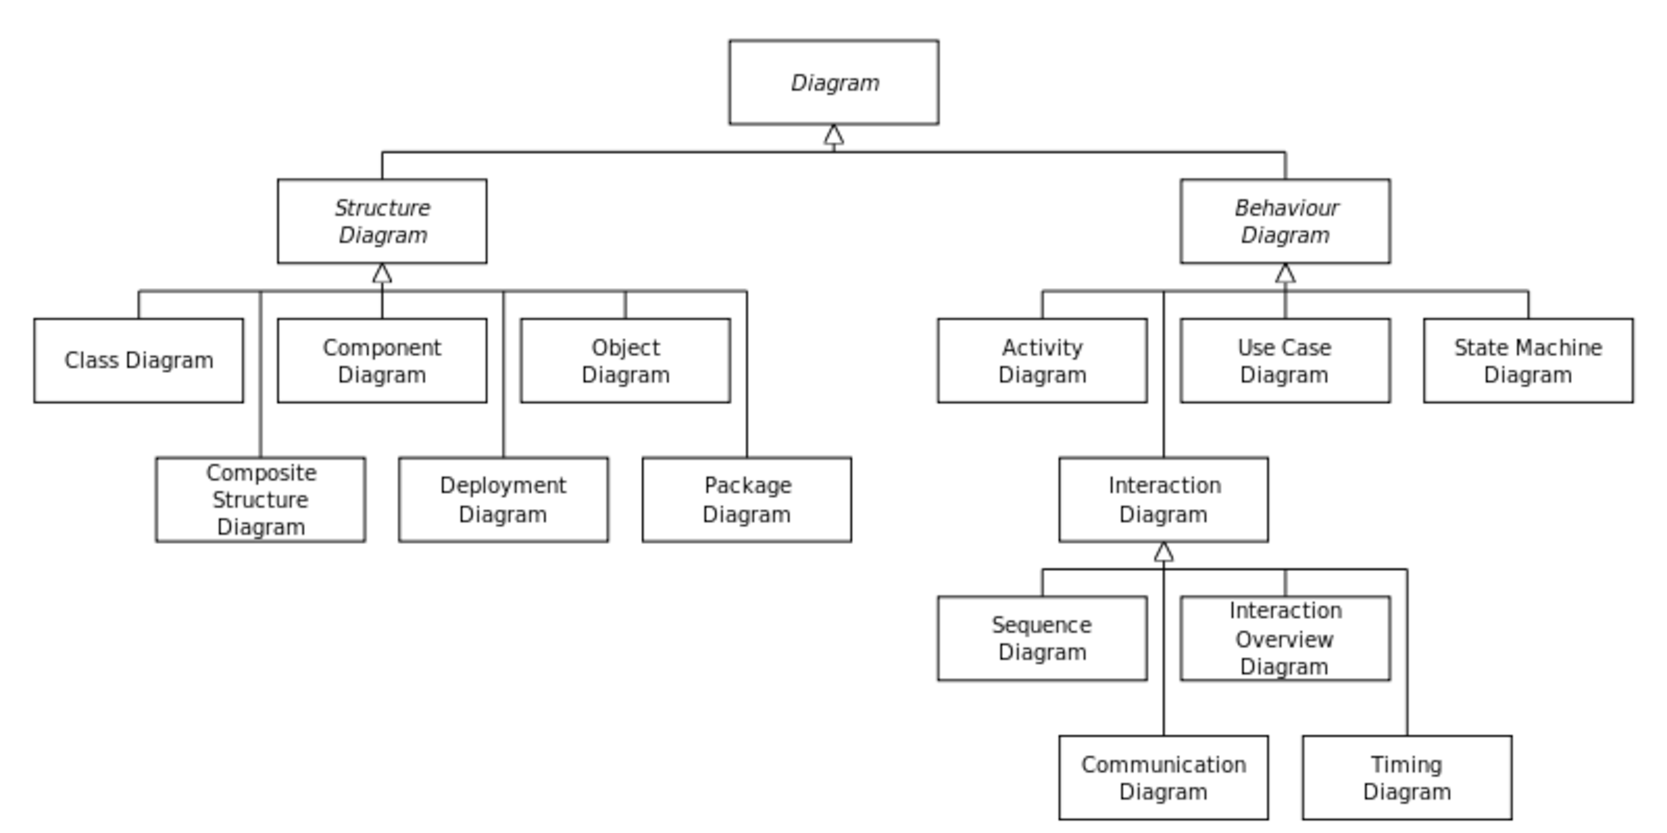
\includegraphics[width=16cm]{exemploFig}
\caption{Exemplo de Figura (\textit{in} \url{http://en.wikipedia.org/wiki/Class_diagram})}
\label{fig:exemplofig}
\end{figure}

Exemplos de citações \cite{AndroidDoc},
\cite{Huetal2000,book:Brooks1995,Chen1976}

%Exemplo de listagem de código Java.
%\lstlisting{

\section{Exemplos de Listagens}

A Listagem \ref{lst:py} apresenta um exemplo de implementação do algoritmo de ordenação \textit{quicksort} na linguagem de programação Python.

\begin{lstlisting}[language=python,caption={Exemplo de listagem de código Pythonescrito directamente no ficehiro tex (apenas recomendado para 1 a 5 linhas de código},{label=lst:py}]
# in http://www.ics.uci.edu/~eppstein/161/python/quicksort-inplace.py - 2013/04/14
# quick sort, in-place 3-way partition
# David Eppstein, UCI, 17 Jan 2002
def swap(A,i,j):
	temp = A[i]
	A[i] = A[j]
	A[j] = temp
\end{lstlisting}


A Listagem \ref{lst:java} apresenta um exemplo de implementação do algoritmo de ordenação \textit{quicksort} na linguagem de programação \Java{}.

\lstinputlisting[language=java,caption={Exemplo de listagem de código Java importado de um ficheiro na pasta listagens.},{label=lst:java}]{listagens/quicksort.java}

\lstinputlisting[language=java,caption={Exemplo de listagem de parte de um ficheiro Java na pasta listagens.},{label=lst:javaparcial},firstline=38,lastline=44]{listagens/quicksort.java}


\pagebreak % para forçar uma mudança de página
%%%%%%%%%%%%%%%%%%%%
\section{Um exemplo de tabela}

A Tabela \ref{tab:caso} apresenta os resultados de aplicação de quatro métodos a um caso.

%baseado num exemplo em http://www1.maths.leeds.ac.uk/latex/TableHelp1.pdf
\begin{table}[htb]
\caption{Uma tabela de exemplo} % título da tabela
\centering % para centrar a tabela
\begin{tabular}{l l c r} % duas colunas à esquerda (l l), uma ao centro (c) e uma à direita (r) (4 colunas)
\hline\hline %insere duas linhas horizontais
Caso & Método 1 & Método 2 & Método 3 \\ [0.5ex] % insere tabela 
\hline % insere uma linha horizontal
1 & 50 & 837 & 970 \\ % insure corpo da tabela
2 & 47 & 877 & 230 \\
3 & 31 & 25 & 415 \\
4 & 35 & 144 & 2356 \\
5 & 45 & 300 & 556 \\ [1ex] % [1ex] adiciona espaço vertical
\hline %insere uma linha horizontal
\end{tabular}
\label{tab:caso} % é utilizada para referir a tabela no texto
\end{table}





%\chapter{Título do Capítulo 3}
\label{cap3}

Mais umas citações \cite{AndroidDoc, Chen1976}

%a linha seguinte deve ser substituída pelo texto do capítulo
\lipsum


% para adicionar o  capítulo N adicione a linha \input{capituloN} e crie o ficheiro
% capituloN.tex na directoria "capitulos"

%%%%%%%%%%%%%%%%%%%%%%%%%%%%%%%%%%%%%%%%%%%%%%%%
% Bibliografia
\clearpage
\printbibliography[heading=bibintoc]
%%%%%%%%%%%%%%%%%%%%%%%%%%%%%%%%%%%%%%%%%%%%%%%%
\apendices
\chapter{Título do Apêndice I}
\label{ap1}

%a linha seguinte deve ser substituída pelo texto do apêndice
\lipsum
% para adicionar o  apêndice N adicione a linha \input{apendiceN} e crie o ficheiro
% apendiceN.tex na directoria "apendices"
%%%%%%%%%%%%%%%%%%%%%%%%%%%%%%%%%%%%%%%%%%%%%%%%
\anexos
\chapter{Implementação do \texttt{parseParamsWebshop}}\label{an1}

\lstinputlisting[frame=bt,language=java,caption={parseParamsWebshop()}]{listagens/parseParamsWebshop.java}
% para adicionar o  anexo N adicione a linha \input{anexoN} e crie o ficheiro
% anexoN.tex na directoria "anexos"
%%%%%%%%%%%%%%%%%%%%%%%%%%%%%%%%%%%%%%%%%%%%%%%%
\end{document}
